%%%%%%%%%%%%%%%%%%%%%%%%%%%%%%%%%%%%
% Slide options
%%%%%%%%%%%%%%%%%%%%%%%%%%%%%%%%%%%%

% Option 1: Slides with solutions

\documentclass[slidestop,compress,mathserif]{beamer}
\newcommand{\soln}[1]{\textit{#1}}
\newcommand{\solnGr}[1]{#1}

% Option 2: Handouts without solutions

%\documentclass[11pt,containsverbatim,handout]{beamer}
%\usepackage{pgfpages}
%\pgfpagesuselayout{4 on 1}[letterpaper,landscape,border shrink=5mm]
%\newcommand{\soln}[1]{ }
%\newcommand{\solnGr}{ }

%%%%%%%%%%%%%%%%%%%%%%%%%%%%%%%%%%%%
% Style
%%%%%%%%%%%%%%%%%%%%%%%%%%%%%%%%%%%%
\def\chp7@path{../../Chp 7}
\input{../../lec_style.tex}


%%%%%%%%%%%%%%%%%%%%%%%%%%%%%%%%%%%%
% Preamble
%%%%%%%%%%%%%%%%%%%%%%%%%%%%%%%%%%%%

\title[Lecture 29]{MA213: Lecture 29}
\subtitle{Module 4: Inference}
\author{OpenIntro Statistics, 4th Edition}
\institute{$\:$ \\ {\footnotesize Based on slides developed by Mine \c{C}etinkaya-Rundel of OpenIntro. \\
The slides may be copied, edited, and/or shared via the \webLink{http://creativecommons.org/licenses/by-sa/3.0/us/}{CC BY-SA license.} \\
Some images may be included under fair use guidelines (educational purposes).}}
\date{}


%%%%%%%%%%%%%%%%%%%%%%%%%%%%%%%%%%%%
% Begin document
%%%%%%%%%%%%%%%%%%%%%%%%%%%%%%%%%%%%

\begin{document}


%%%%%%%%%%%%%%%%%%%%%%%%%%%%%%%%%%%%
% Title page
%%%%%%%%%%%%%%%%%%%%%%%%%%%%%%%%%%%%

{
\addtocounter{framenumber}{-1} 
{\removepagenumbers 
\usebackgroundtemplate{\includegraphics[width=\paperwidth]{../../OpenIntro_Grid_4_3-01.jpg}}
\begin{frame}

\hfill \includegraphics[width=20mm]{../../oiLogo_highres}

\titlepage

\end{frame}
}
}


%%%%%%%%%%%%%%%%%%%%%%%%%%%%%%%%%%%%
% Recap/Agenda 
%%%%%%%%%%%%%%%%%%%%%%%%%%%%%%%%%%%%
% TODO better formatting
\begin{frame}
    \frametitle{Module 4: Inference}
    \begin{itemize}
        \item \hl{Previously: }Comparing many means with ANOVA (Chapter 7.5)
        \item \hl{This time: }Issues with Hypothesis Testing 2: Multiple comparisons
        \item \hl{Reading: }Chapter 8.1 for next time
        \item \hl{Deadlines/Announcements: }HW 4.3 due Monday
    \end{itemize}
    
\end{frame}
%%%%%%%%%%%%%%%%%%%%%%%%%%%%%%%%%%%%
% Sections
%%%%%%%%%%%%%%%%%%%%%%%%%%%%%%%%%%%%

%%%%%%%%%%%%%%%%%%%%%%%%%%%%%%%%%%%

\section{Review} % TODO: ANOVA recap slides


%%%%%%%%%%%%%%%%%%%%%%%%%%%%%%%%%%%

\subsection{Multiple comparisons \& Type 1 error rate}

%%%%%%%%%%%%%%%%%%%%%%%%%%%%%%%%%%%

\begin{frame}
\frametitle{Which means differ?}

\begin{itemize}

\item Earlier we concluded that at least one pair of means differ. The natural question that follows is ``which ones?"

\pause

\item We can do two sample $t$ tests for differences in each possible pair of groups.

\pause

\end{itemize}

\dq{Can you see any pitfalls with this approach?}

% \pause

% \begin{itemize}

% \item When we run too many tests, the Type 1 Error rate increases.

% \item This issue is resolved by using a modified significance level.

% \end{itemize}

\end{frame}

%%%%%%%%%%%%%%%%%%%%%%%%%%%%%%%%%%%

\begin{frame}
\begin{center}
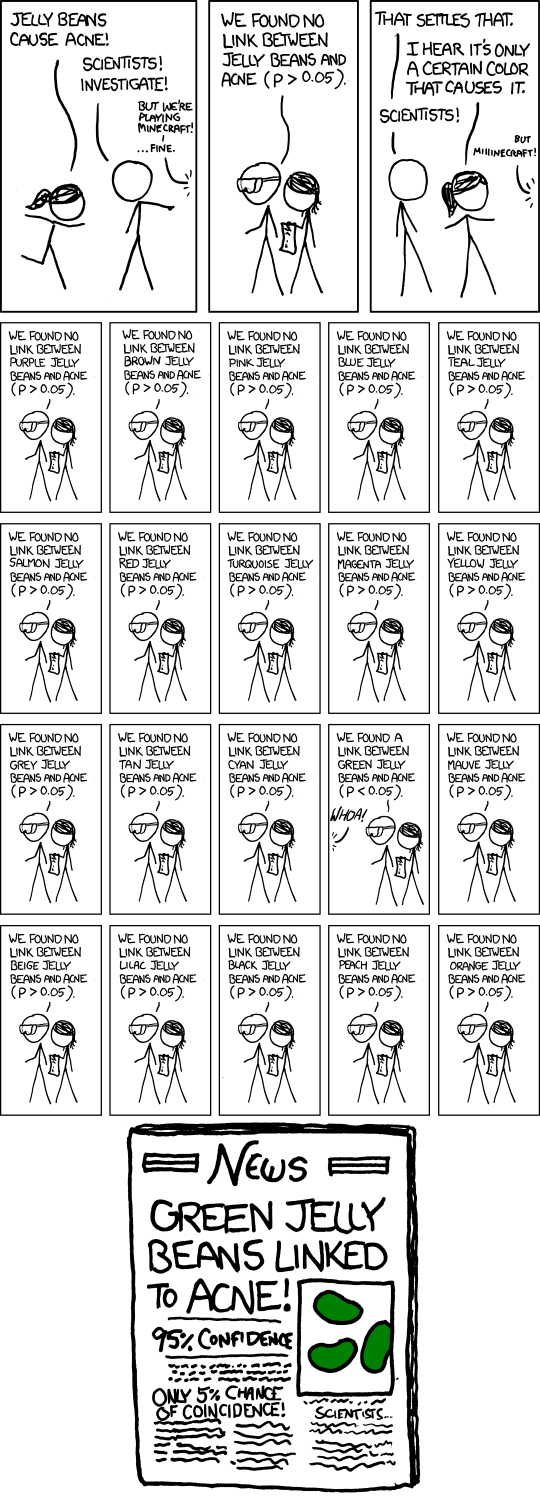
\includegraphics[width=0.9\textwidth]{xkcd_significance.png}
\end{center}
\end{frame}

%%%%%%%%%%%%%%%%%%%%%%%%%%%%%%%%%%%

\begin{frame}
\begin{center}
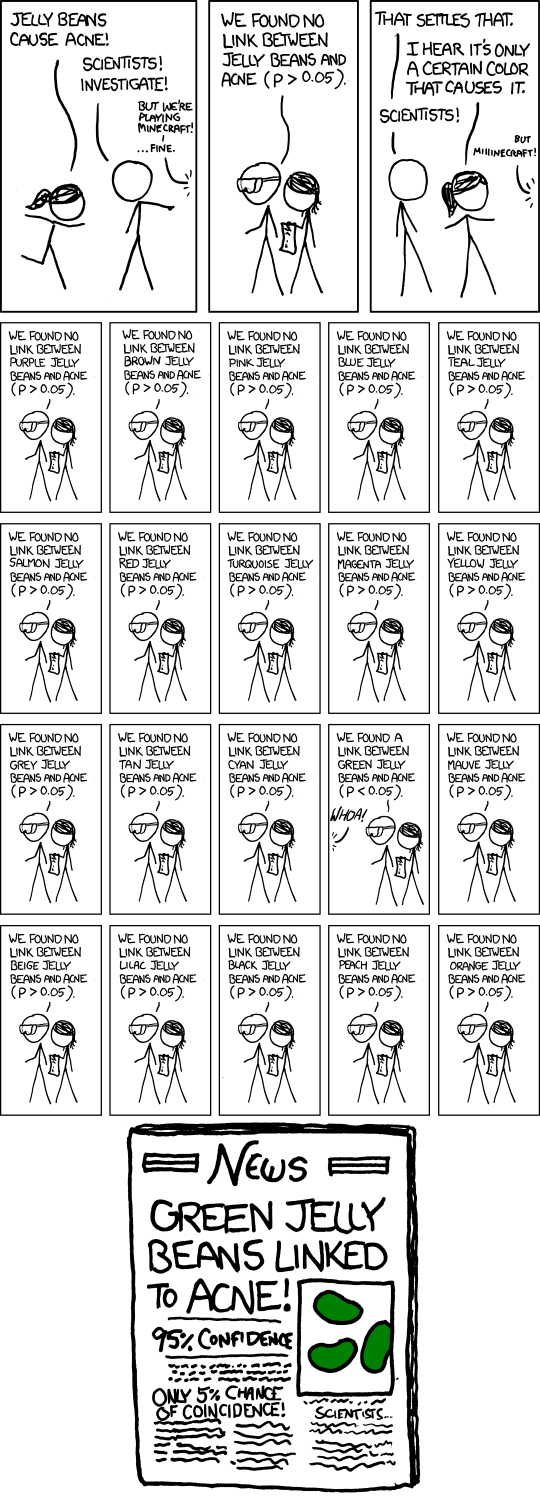
\includegraphics[height=0.95\textheight]{xkcd_significance.png}
\end{center}

\footnotesize https://imgs.xkcd.com/comics/significant.png
\end{frame}

%%%%%%%%%%%%%%%%%%%%%%%%%%%%%%%%%%%

\begin{frame}
\frametitle{Multiple comparisons}

\begin{itemize}

\item The scenario of testing many pairs of groups is called \hl{multiple comparisons}.

\pause

\item The \hl{Bonferroni correction} suggests that a more \orange{stringent} significance level is more appropriate for these tests:

\[ \alpha^\star = \alpha / K \]

where $K$ is the number of comparisons being considered.

\pause

\item If there are $k$ groups, then usually all possible pairs are compared and $K = \frac{k (k - 1)}{2}$.

\end{itemize}

\end{frame}

%%%%%%%%%%%%%%%%%%%%%%%%%%%%%%%%%%%

\begin{frame}
\frametitle{Determining the modified $\alpha$}

\pq{In the aldrin data set depth has 3 levels: bottom, mid-depth, and surface. If $\alpha = 0.05$, what should be the modified significance level for two sample $t$ tests for determining which pairs of groups have significantly different means?}

\begin{enumerate}[(a)]
\item $\alpha^* = 0.05$
\item $\alpha^* = 0.05 / 2 = 0.025$
\solnMult{$\alpha^* = 0.05 / 3 = 0.0167$}
\item $\alpha^* = 0.05 / 6 = 0.0083$
\end{enumerate}

\end{frame}

%%%%%%%%%%%%%%%%%%%%%%%%%%%%%%%%%%%

\begin{frame}
\frametitle{Which means differ?}

\pq{Based on the box plots below, which means would you expect to be significantly different?}

\twocol{0.6}{0.4}{
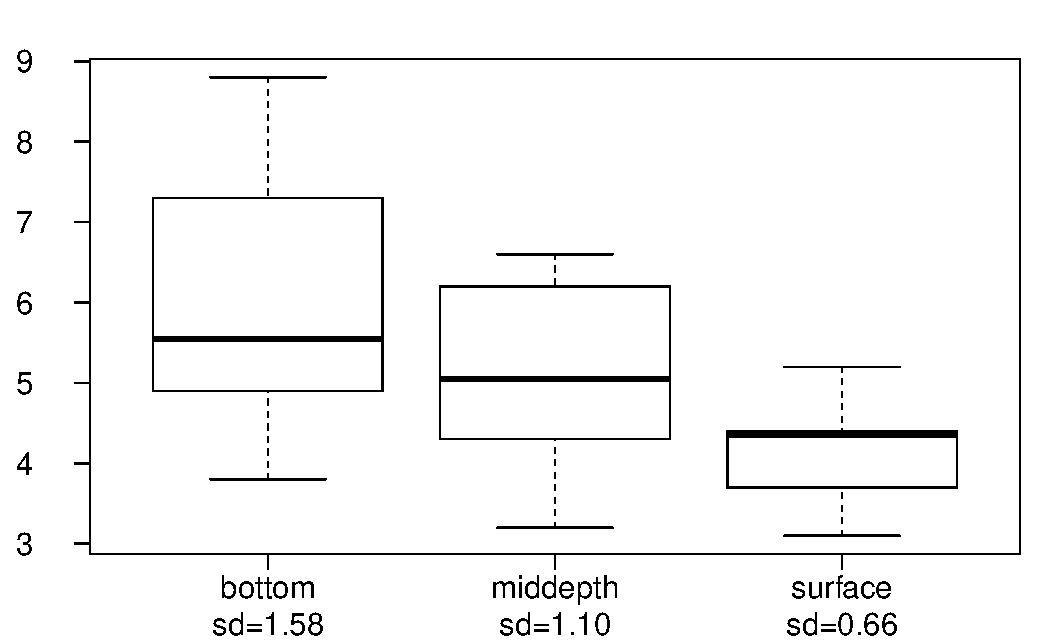
\includegraphics[width=\textwidth]{\chp7@path/7-5_anova/figures/aldrin/homo}
}
{
\begin{enumerate}[(a)]
\item bottom \& surface
\item bottom \& mid-depth
\item mid-depth \& surface
\item bottom \& mid-depth; mid-depth \& surface
\item bottom \& mid-depth; bottom \& surface; mid-depth \& surface
\end{enumerate}
}

\end{frame}

%%%%%%%%%%%%%%%%%%%%%%%%%%%%%%%%%%

\begin{frame}
\frametitle{Which means differ? (cont.)}

If the ANOVA assumption of equal variability across groups is satisfied, we can use the data from all groups to estimate variability:
    
\begin{itemize}

\item Estimate any within-group standard deviation with $\sqrt{MSE}$, which is $s_{pooled}$

\item Use the error degrees of freedom, $n - k$, for $t$-distributions

\end{itemize}

\formula{Difference in two means: after ANOVA}{
\[ SE = \sqrt{  \frac{\sigma_1^2}{n_1} + \frac{\sigma_2^2}{n_2} } \approx \sqrt{ \frac{MSE}{n_1} + \frac{MSE}{n_2} } \]
}

\end{frame}

%%%%%%%%%%%%%%%%%%%%%%%%%%%%%%%%%%

\begin{frame}
\frametitle{}

\dq{Is there a difference between the  average aldrin concentration at the bottom and at mid depth?}

\twocol{0.4}{0.7}{
{\scriptsize
\begin{center}
\begin{tabular}{l | c c c}
        & n	& mean	& sd		\\
\hline
bottom	& 10	& \orange{6.04}	& 1.58 \\
middepth& 10	& \orange{5.05}	& 1.10 \\
surface	& 10	& 4.2 	& 0.66 \\
\hline
overall	& 30	& 5.1		& 1.37
\end{tabular}
\end{center}
}
}
{
{\scriptsize
\begin{center}
\begin{tabular}{l rrrrr}
\hline
                & Df 	& Sum Sq	& Mean Sq 	& F value 	& Pr($>$F) \\ 
\hline
depth 		& 2 	& 16.96 	& 8.48 		& 6.13 	& 0.0063 \\ 
Residuals 	& \orange{27} 	& 37.33 	& \orange{1.38} 		&  		&  \\ 
\hline
Total			& 29	& 54.29 \\
\end{tabular}
\end{center}
}
}

\begin{eqnarray*}
T_{df_E} &=& \frac{(\bar{x}_{bottom} - \bar{x}_{middepth})}{\sqrt{ \frac{MSE}{n_{bottom}} + \frac{MSE}{n_{middepth}} }} \\ 
\pause
T_{27} &=& \frac{( 6.04 - 5.05 )}{\sqrt{ \frac{1.38}{10} + \frac{1.38}{10} }} = \frac{0.99}{0.53}  =1.87 \\
\pause
0.05 &<& p-value < 0.10 \qquad \text{{\footnotesize (two-sided)}} \\
\pause
\alpha^\star &=& 0.05 / 3 = 0.0167
\end{eqnarray*}

\pause
{\small Fail to reject $H_0$, data do not provide convincing evidence of a difference between average aldrin concentrations at bottom and mid depth.}

\end{frame}

%%%%%%%%%%%%%%%%%%%%%%%%%%%%%%%%%%

\begin{frame}
\frametitle{}

\app{Pairwise comparisons}{Is there a difference between the  average aldrin concentration at the bottom and at surface?}

\pause

\soln{
\begin{eqnarray*}
T_{df_E} &=& \frac{(\bar{x}_{bottom} - \bar{x}_{surface})}{\sqrt{ \frac{MSE}{n_{bottom}} + \frac{MSE}{n_{surface}} }} \\ 
\pause
T_{27} &=& \frac{( 6.04 - 4.2 )}{\sqrt{ \frac{1.38}{10} + \frac{1.38}{10} }} = \frac{1.84}{0.53}  =3.47 \\
\pause
p-value = 0.0018 \qquad \text{{\footnotesize (two-sided)}} \\
\pause
\alpha^\star &=& 0.05 / 3 = 0.0167
\end{eqnarray*}
\pause
{\small Reject $H_0$, the data provide convincing evidence of a difference between the average aldrin concentrations at bottom and surface.}
}

\end{frame}

%%%%%%%%%%%%%%%%%%%%%%%%%%%%%%%%%%

%%%%%%%%%%%%%%%%%%%%%%%%%%%%%%%%%%    


%%%%%%%%%%%%%%%%%%%%%%%%%%%%%%%%%%%%
% End document
%%%%%%%%%%%%%%%%%%%%%%%%%%%%%%%%%%%%

\end{document}